\textbf{Цель работы:} определение коэффициента поверхностного натяжения методом <<Разрыва тонкого слоя жидкости>>.

\textbf{Принадлежности:} кольцо для изучения поврхностного натяжения, точный динамометр $(0.1H)$, стакан из комплекта дополнительного оборудования, лабораторный подъёмный столик со штативом из нержавеющей стали и крючком, штангенциркуль.Установка (рис.\ref{fig:installation})

\begin{figure}[!h]
    \centering
    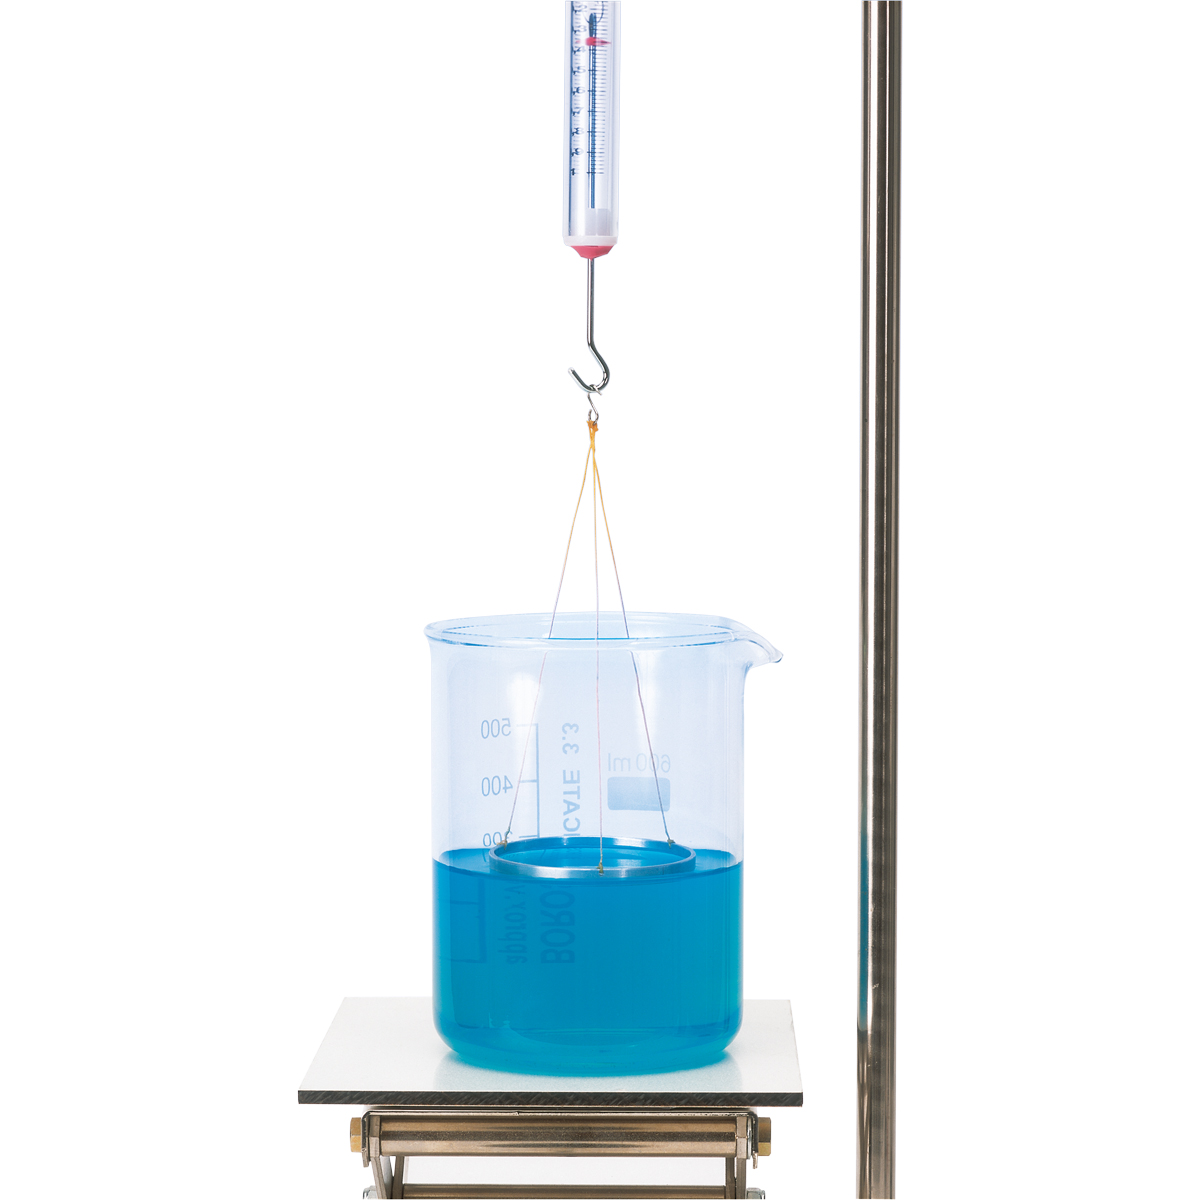
\includegraphics[width = 0.5\textwidth]{image/image.png}
    \caption{установка}
    \label{fig:installation}
\end{figure}

\textbf{Вывод рабочей формулы:}

Поверхностное натяжение жидкости "--- это её свойство на границе контакта с окружающей средой. Оно обусловлено тем, что молекула жидкости, находящаяся на её поверхности, испытывает действие сил со стороны соседних с ней молекул жидкости только из половины пространства, ограниченной поверхностью этой жидкости, в то время как молекула внутри жидкости испытывает воздействие со всех сторон. Поэтому молекула в поверхностном слое испытывает воздействие результирующей силы, направленной перпендикулярно к поверхности внутрь жидкости.

Действие этой силы приводит к сокращению площади поверхности жидкости. Взаимодействие молекул в поверхностном слое также обуславливает наличие горизонтальной составляющей сил, способствующей стремлению площади поверхности к сокращению. Эти силы получили название сил поверхностного натяжения. Сила поверхностного $F_\text{н}$ натяжения направлена по касательной к поверхности жидкости. За счёт воздействия сил поверхностного натяжения молекулы жидкости в поверхностном слое обладаююь дополнительной потенциальной энергией по сравнению с молекулами внутреннего объема. Это дополнительная энергия называется поверхностной энергией $W_\text{пов}$ и пропорциональна площади поверхности жидкости:

\begin{equation*}
    W_\text{пов} = \alpha S
\end{equation*}

Коэффициент пропорциональности $\alpha$ является мерой свободной поверхности.

\begin{equation*}
    \alpha = \frac{W_\text{пов}}{S}
\end{equation*}

называется коэффициентом поврхностного натяжения и зависит от природы и состояния как жидкости, так и той среды с которой соприкасается её поверхность. То есть от физико"=химических свойств, определяющих энергию взаимодействия их молекул.

Физический смысл коэффициента поверхностного натяжения состоит в том, что он численно равен рабооте, затрачиваемой на образование $1 \text{м}^2$ поверхности жидкости при постоянной температуре.

\begin{equation*}
    \alpha = \frac{d A_\text{пов}}{d S}
\end{equation*}

и представляет собой силу сцепления поверхностной плёнки жидкости. Вызванную взаимным притяжением молекул, находящихся по обе стороны линии контура её разрыва, дейстующую на единицу длины:

\begin{equation*}
    F_\text{н} = \alpha L
\end{equation*}

Определить коэффициент поверхностного натяжения можно увеличив поверхность жидкости на величин $d S$ переводом в поверхностный слой некоторого числа молекул, совершив тем самым работы $d A_\text{пов}$. Осуществить это возможно при помощи кольца с острой кромкой, которое изначально полностью погружено в жидкость. Если, приложив внешнюю силу $F_\text{вн}$, компенсирующую силу поверхностного натяжения $F_\text{вн}$, кольцо медленно извлеать из жидкости, тонкий слой жидкости вытягивается вверх за его нижним краем (рис. \ref{fig:installation})

\begin{equation*}
    d A_\text{пов} = F_\text{вн} \Delta x
\end{equation*}

Когда кольцо поднимается на высоту $\Delta x$, площадь поверхности тонкого слоя увеличивается снаружи и внутри кольца в общем на:

\begin{equation*}
    d S = 4 \pi R \Delta x
\end{equation*}

где $R$ "--- радиус кольца. 

Если сила $F_\text{вн}$, прилагаемая при подъёме кольца, превышает $F_\text{н}$, тонкий слой жидкости рвется. В этот момент можно определить:

\begin{equation}
    \alpha = \frac{F_\text{вн}}{4 \pi R}
    \label{eq : alpha}
\end{equation}

\vspace{0.5cm}

\textbf{Описание установки:}

В этой работе металлическое кольцо с острой нижней кромкой свисает в горизонтальном положении с точного динамометра. Сначала кольцо полностью погружено в испытываемую жидкость (например, в воду), затем оно медленно извлекается из жидкости. Тонкий слой жидкости разрывается, когда сила вытягивания $F_\text{вн}$, превышает предельное значение $F_\text{н}$.

\vspace{0.5cm}

\textbf{Порядок выполнения работы:}
\begin{enumerate}
    \item {Установить лабораторный подъёмный столик на минимальный уровень подъёма.}
    \item {Подвесить динамометр на вертикальный штатив с крючком.}
    \item {Измерить диаметр кольца и подвесить его к динамометру.Значения диаметра занести в таблицу.}
    \item {Наполнить стакан исследуемой жидкостью и поставить его на лабораторный подъёмный столик.}
    \item {Поднять стакан подъёмным столиком до погружения в жидкость острой нижней кромки кольца.}
    \item {Записать показание динамометра $F_1$ в таблицу}
    \item {Медленно опустить лабораторный подъёмный столик со стаканом до момента разрыва пленки (отрыва кольца от жидкости).}
    \item {В момент разрыва снять показание динамометра $F_2$ и занесите в таблицу}
    \item {
        Рассчитать и занести в таблицу \ref{tab:my_label} разницу между двумя значениями силы:
        \begin{equation*}
            F_\text{вн} = F_2 - F_1
        \end{equation*}
    }
    \item {Повторить измерение несколько раз и проверить воспроизводимость.}
    \item {Используя полученные данные, вычислить по формуле \ref{eq : alpha} значение коэффициента поверхностного натяжения $\alpha$ исследуемой жидкости для каждого измерения и занести в таблицу}
    \item {Определить среднее значение коэффициента поверхностного натяжения $\alpha _\text{ср}$, абсолютною погрешность $\Delta \alpha$ и среднее значение абсолюной погрешности $\Delta \alpha _\text{ср}$.Занести полученные данные в таблицу \ref{tab:my_label} (Значение коэфициента поверхностного натяжения эталонной жидкости $\Delta \alpha _\text{табл}$ для расчетов взять из справочных данных.)}
    \item {Записать полученный результат в таблицу $\alpha _\text{ср} \pm \Delta \alpha _\text{ср}$.}
    \item {
        Вычислить относительную погрешность измерений {$\delta$} по формуле:
        \begin{equation*}
            \delta = \frac{\delta \alpha _ \text{ср}}{\alpha _ \text{ср}} \cdot 100\% 
        \end{equation*}
    }
    \item {
        Сравнить полученное значение коэффициента поверхностного натяжения с его табличным значением. Сравнить расхождение экспериментально полученного и табличного значений по формуле:
        \begin{equation*}
            \Delta \sum =  \left(\frac{| \alpha _\text{ср} - \alpha _\text{табл}|}{\alpha _\text{табл}} \right) \cdot 100\%
        \end{equation*}
    }
\end{enumerate}
    
\[\ln{\alpha}=\ln{F_{vn}} - \ln{4\pi} - \ln{R}\]\
\[d\alpha= d F_{vn} - d R\]

\[|\frac{\Delta \alpha}{\alpha}| = |\frac{\Delta F_{vn}}{F_{vn}}| + |\frac{\Delta R}{R}|\]

\[|\frac{\Delta \alpha}{\alpha}| = (|\frac{0,001}{0,02}| + |\frac{1}{30}|) \cdot 100 \% = (|\frac{1}{20}| + |\frac{1}{30}|) \cdot 100 \% = 8,3 \%\]

\begin{table}[!h]
    \centering
    \resizebox{\textwidth}{!}{
    \begin{tabular}{|c|c|c|c|c|c|c|c|c|c|c|c|c|}
         \hline
         %первая часть превой строки
         \makecell{№\\опы\\та} &
         \makecell{Диам\\етр\\коль\\ца\\$D_\text{к}$,м}&
         \multicolumn{2}{|c|}{\makecell{Пока\\зания\\динамо\\метра}}&
         \makecell{Дейст\\вую\\щая\\сила\\$F_\text{вн}$, H}&
         \multicolumn{3}{|c|}{\makecell{Коэффициэнт\\поверхностного\\натяжения}}&
         \multicolumn{3}{|c|}{\makecell{Погрешность\\изменения}}&
        \makecell{Полу\\ченный\\резуль\\тат\\$\alpha _\text{ср} \pm$\\$ \Delta \alpha _\text{ср}$} &
         \makecell{Расхож\\дение с\\таблич\\ным зна\\чением\\$\Delta \sum $,$ \%$}\\
         %вторая часть первой строки
         \cline{3-4}\cline{6-8}\cline{9-11}
         & & \makecell{$F_1 $,\\H}& \makecell{$F_2 $,\\H}& &
         \makecell{Изме\\рен\\ный\\$\alpha $,$\frac{H}{\text{м}}$}&
         \makecell{Сред\\нее\\$\alpha _\text{ср}$,\\$\frac{H}{\text{м}}$}&
         \makecell{Таб\\лич\\ный\\$\alpha _\text{табл}$,\\$\frac{H}{\text{м}}$}&
         \makecell{Абсо\\лют\\ная\\$\Delta \alpha$,\\$\frac{H}{\text{м}}$}&
         \makecell{Сред\\нее\\$\Delta \alpha _\text{ср}$,\\$\frac{H}{\text{м}}$}&
         \makecell{Отно\\ситель\\ная\\$\delta$,$\%$}& &\\
         \hline
         1& & \makecell{0.051}& \makecell{0.072}& \makecell{0.021}& \makecell{0.056}& & & \makecell{0.015}& & & & & 
         \cline{1-1}\cline{3-6}\cline{9-9}
         2& & \makecell{0.052}& \makecell{0.073}& \makecell{0.021}& \makecell{0.056}& & & \makecell{0.015}& & & & &
         \cline{1-1}\cline{3-6}\cline{9-9}
         
         3& \makecell{0.06}& \makecell{0.051}& \makecell{0.073}& \makecell{0.022}& \makecell{0.058}& \makecell{0.055}& \makecell{0.071}& \makecell{0.013}& \makecell{0.0158}& \makecell{1.81}& \makecell{0.055\\$\pm$\\0.0158}& \makecell{22.53}&
         
         \cline{1-1}\cline{3-6}\cline{9-9}
         4& & \makecell{0.052}& \makecell{0.072}& \makecell{0.02}& \makecell{0.053}& & & \makecell{0.018}& & & & &
         \cline{1-1}\cline{3-6}\cline{9-9}
         5& & \makecell{0.052}& \makecell{0.072}& \makecell{0.02}& \makecell{0.053}& & & \makecell{0.018}& & & & &
         \hline
    \end{tabular}
    }
    \caption{Измерения}
    \label{tab:my_label}
\end{table}

\textbf{Вывод:}

Определили коэффициент поверхностного натяжения воды методом разрыва тонкого слоя жидкости. Нашли относительную погрешность коэффициента поверхностного натяжения воды и рассчитали расхождение с табличным значением коэффициента поверхностного натяжения.

Максимальная погрешность больше экпериментальной (\(8,3 \% > 1,81 \%\) ), что означает, что опыт проведён правильно.

